\chapter[On the Newtonian spacetime and a 4-vector formulation...]{On the Newtonian spacetime and a 4-vector formulation of the Newton law of motion}\label{chap16}

\Authorline{A V Gopala Rao,}

\authinfo{Department of  Studies in Physics,\\
University of Mysore, Manasagangotri,\\
Mysuru 570006, India
}

\noindent
Professor G Ramachandran was my senior colleague at the Department of Physics, University of Mysore.~With pleasure and humility, I dedicate this article to the memory of the learned Professor.

\begin{abstract} 
We discuss a tensor-geometric formulation of the Newton law of motion.\\[3pt]
\textsl{Professor G Ramachandran was my senior colleague at the Department of Physics, University of Mysore. With pleasure and humility, I dedicate this article to the memory of the learned Professor.}
\end{abstract}

\noindent
\textsl{Notation}: Latin suffixes  $i,j,k,..$, are used for the spacetime range $0,1,\break 2,3$ and Greek suffixes  $\alpha, \beta, \gamma, ..$, for the spatial  range $1,2,3$. Special upper case bold-symbols such as $\tns{T}, \tns{N}, \tns{U},\tns{A},\dt$,  denote 4-vectors in the Newtonian spacetime $\mbb{N}$.  Spatial-3-vectors are denoted by an over-head arrow as in $\veca{r}$,  $\veca{v}$,  $\veca{a}$, $\veca{f}$ etc. Bold-upper-case characters such as $\bmsf{T,N,U,A,F},\dt$, denote 4-dimensional matrices and 4-dimensional column-matrices. Bold-lower-case characters such as $\bmsf{u,a,p,f},\dt$, denote 3-dimensional matrices and 3-dimensional column matrices.  An over-head ``tilde'' as in $\wt{\bmsf{A}}$ or  $\wt{\bmsf{a}}$ denote the transposes of the matrices  $\bmsf{A}$ and $\bmsf{a}$. Superscripts and subscripts, as in  $T^i$ and  $N_i$, are contravariant and covariant indices. A semicolon as in $N_{i;j}$ indicates  covariant differentiation with respect to the \textsl{affinity} in the Newtonian spacetime $\mbb{N}$.

\section{Introduction}\label{chap16-sec1}

The Minkowskian nature of the geometry of the spacetime of the special theory of relativity, and the general Riemannian nature of the geometry of the spacetime of the general theory of relativity, are well known. This makes a mathematically inclined student of physics  wonder if absolute space and absolute time which occur as independent geometric entities in Newtonian Mechanics, may similarly be combined together into a 4-dimensional geometric continuum, and if so, what could be the geometric nature of such a  Newtonian spacetime. As an  answer to that query, we present in this article elements of the geometry of the Newtonian spacetime as discussed in Anderson's book \cite{chap16-key1} and, as an application of the method, discuss, very briefly, the Newtonian mechanics of a particle in accelerated frames of reference.

\section{The Newtonian spacetime}\label{chap16-sec2}

The geometry of the \textsl{Newtonian spacetime} $\mathbb{N}$ is described in detail in Anderson's book [1, pp.106-110]. Here, we quote  the essential elements of that discussion.

The \textsl{Newtonian spacetime} is a real 4-dimensional manifold  $\mathbb{N}$ endowed with a \textbf{symmetric flat affinity\footnote{The affinity is flat in the sense that the associated Riemann tensor is zero on $\mbb{N}$.}} $\bmsf{\Gamma}$, a covariant 4-vector field $\tns{N}$,  and a contravariant 4-vector field  $\tns{T}$. These objects $\bmsf{\Gamma}$, $\tns{N}$ and $\tns{T}$, are assumed to be defined   at all points of $\mathbb{N}$. As in relativity theory, points of $\mathbb{N}$ may be  called \textsl{events}. 

Furthermore, it is  assumed that the vector fields $\tns{N}$ and $\tns{T}$ satisfy the conditions 
\setcounter{equation}{0}
\begin{equation}
T^i N_i =1,\quad  N_{i;j}=0, \quad  T^i_{\;;j}=0, \quad  \partial_i  N_j - \partial_j N_i=0,\label{chap16-eq1} 
\end{equation}
at every event of $\mbb{N}$. Above,  the partial  and covariant derivatives are defined in the usual way by
\begin{equation*}
\partial_i  N_j\equiv \partial N_j/\partial x^i,\quad T^i;j\equiv\partial_j  T^i+\Gamma^i_{kj} T^k,\quad N_{i;j}\equiv\partial_j  N_i-\Gamma^k_{ij} N_k,
\end{equation*}
where $\Gamma^k_{ij}$ are the coefficients of the symmetric affinity $\bmsf{\Gamma}$ in the coordinate system $\{x^i\}$. From Eqn.~\eqref{chap16-eq1}, it is clear that $\tns{N}$ and $\tns{T}$ are covariantly constant vector fields. Further, one can introduce [Anderson,1] a \textsl{global canonical coordinate System} 
\begin{equation}
\{x^i\}\equiv \{x^0\equiv t, x^1\equiv x,x^2\equiv y,x^3\equiv z\} \label{chap16-eq2}
\end{equation}
in  $\mbb{N}$  in which 
\begin{equation*}
\Gamma^i_{jk}=0, \quad T^i=(1,0,0,0),\quad N_i=(1,0,0,0),\tag{2b}\label{chap16-eq2b}
\end{equation*}
\textbf{at all events of} $\mbb{N}$. Observe that the covariant components $N_i$ of $\tns{N}$ given in Eqn.~\eqref{chap16-eq2b} may be expressed as  
\begin{equation*}
N_i=t_{;i} \equiv (\partial t/\partial x^i)=(1,\;0,\;0,\;0).\tag{2c}\label{chap16-eq2c}
\end{equation*}
This is the necessary and sufficient condition for $\tns{N}$ to be  a \textsl{hypersurface orthogonal} 4-vector field: Clearly, in the canonical coordinate system $\{x^i\}$  in Eqn.~\eqref{chap16-eq2}, $N_i$ is normal to the 3-dimensional hypersurfaces $t=\textsl{constant}$. The 3-dimensional hypersurfaces  $t=\textsl{constant}$  are called the \textbf{hypersurfaces of absolute simultaneity} in $\mbb{N}$. All events on such a hypersurface of absolute simultaneity occur at the same instant $t$. 

\subsection{Inertial frame}\label{chap16-sec2.1}

The \textsl{global, canonical coordinate system} $\{x^i\}\equiv\{t, x,y,z\} $ mentioned above in Eqn.~\eqref{chap16-eq2} has space-coordinates $\{x,y,z\}$ which are Cartesian. Further, in this canonical coordinate system in Eqn.~\eqref{chap16-eq2}, in which the properties \eqref{chap16-eq2b} and \eqref{chap16-eq2c} are true, all the components of affine connection $\Gamma^i_{jk}$ are zero (showing that this  symmetric affinity $\bmsf{\Gamma}$ is indeed flat). This global, canonical coordinate system in $\mbb{N}$ is called an \textbf{inertial coordinate system} or, an \textbf{inertial frame}. 

It is useful to note that in an inertial frame, the time and space intervals between two events $P:(t_P,x_P,y_P,z_P)$ and $Q:(t_Q,x_Q,y_Q,z_Q)$  are given by
\begin{equation}
(\Delta  t_{PQ})^2=(t_P-t_Q)^2,\label{chap16-eq3}
\end{equation}
and 
\begin{equation}
(\Delta  \ell_{PQ})^2=(x_P-x_Q)^2+(y_P-y_Q)^2+(z_P-z_Q)^2.\label{chap16-eq4}
\end{equation}

\subsection{Non-inertial frame}\label{chap16-sec2.2}

In addition to an inertial frame $\{x^i\}\equiv\{t,x,y,z\}$, coordinate frames  $\{\bar{x}^i\}$ obtained from an inertial frame by a transformation of the type 
\begin{equation}
\bar{x}^i=\bar{x}^i(t, x,y,z),\label{chap16-eq5}
\end{equation}
where $\bar{x}^i (t, x,y,z)$ are arbitrary differentiable functions of the $(t, x,y,z)$,  are also of interest in physics. Of particular importance among these are a sub-class of transformations of the type\footnote{Since we confine ourseleves to considering coordinate transformations of the type (5a) which preserve the absolute time $t$, we write, in what follows $\bar{x}^0=x^0=t$ to simplify the notation.} 
\begin{align*}
& \bar{x}^0= t,\\
& \bar{x}^\alpha=\bar{x}^\alpha(t, x,y,z),\quad \alpha=1,2,3,\tag{5a}\label{chap16-eq5a}
\end{align*}
and this class includes most of the  frames which are of interest in physics. We note that the \textbf{Galilei transformation} 
\begin{equation}
 \bar{x}^0=t,\;\veca{\bar{r}} =\veca{r}-\veca{v_0}t ,\label{chap16-eq6}
\end{equation}
where $\veca{{r}}\equiv  (x,y,z)$, $\veca{\bar{r}}\equiv  (\bar{x}^1,\bar{x}^2,\bar{x}^3)$ and $\veca{v_0}\equiv  (v^1,v^2,v^3)$ is a constant 3-vector, belongs to this class defined in Eqn.~\eqref{chap16-eq5a}. A Galilei transformation, however,  transforms an  inertial frame $\{x^i\}$ into another inertial frame $\{\bar{x}^i\}$. Therefore, if our interest lies in transforming an inertial frame into a non-inertial frame, we must consider non-Galilei transformations. 

\section{4-trajectory, 4-velocity and  4-acceleration}\label{chap16-sec3}

The \textbf{spacetime trajectory or 4-trajectory}  $C$ of a point-particle is a curve in  $\mbb{N}$. In a coordinate system   $\{x^i\}$,  with $x^0\equiv t$, $C$ is described by the parametric equation  $C: x^i=x^i(t)$. A general event on  $C$ at time $t$ would then have the coordinates  $(t,\;x^\alpha (t))$. 

The  \textbf{4-velocity} $\tns{U}$ of the particle is a \textbf{tangent vector} to  $C$. In dealing with the 4-velocity, it is convenient to work with a 4-dimensional column-matrix $\bmsf{U}$ whose elements    are the contravariant components of $\tns{U}$, namely, $U^0=\dd x^0/\dd t=1$, $U^1=\dd x^1/\dd t$, $U^2= \dd x^2/\dd t$, $U^3=\dd x^3/\dd t$ in $\{x^i\}$. Therefore, we have
\setcounter{equation}{6}
\begin{equation}
\tns{U}\mapsto{\bmsf{U}}=(U^i)=(\dd x^i /\dd t)=\left(\begin{array}{c} \dot{x}{}^{0}\\ \dot{x}{}^1\\ \dot{x}{}^2\\\dot{x}{}^3\end{array}\right)=  \left(\begin{array}{c} 1\\ \bmsf{u}\end{array}\right),\label{chap16-eq7}
\end{equation}
where the derivatives $\dot{x}{}^\alpha, \,\alpha= 1,2,3$, are evaluated on $C$ and the 3-column matrix  
\begin{equation}
\bmsf{u}=\left(\begin{array}{c}u^1\\ u^2\\ u^3\end{array}\right) =\left(\begin{array}{c}\dot{x}{}^1\\ \dot{x}{}^2\\ \dot{x}{}^3\end{array}\right),\label{chap16-eq8}
\end{equation}
is called the 3-velocity of the particle. 

The \textbf{4-acceleration}   $\tns{A}$ of a particle is defined as the \textbf{intrinsic derivative} ${\mathrm{D}} \tns{U}/\dd t$ of the 4-velocity $\tns{U}$ along the 4-trajectory $C$ of the particle. Therefore, the contravariant components of the 4-acceleration are 
\begin{equation}
A^i= {\mathrm{D}}U^i /dt=\dd  U^i /\dd t + \Gamma^i _{jk}  U^j U^k ,\label{chap16-eq9}
\end{equation}
which involve the \textsl{affine-coefficients}  $\Gamma^i_{jk}$ in $\{x^i\}$. In particular, in an \textbf{inertial frame} $\{x^i\}\equiv\{t,x,y,z\}$, where $({\mathrm D}U^i/\dd t)=    ( \dd U^i /\dd t)$ because  all the affine-coefficients vanish at all events, we have
\begin{equation}
{\bmsf{A}}=(A^i) =( \dd U^i /\dd t)=\left(\begin{array}{c} 0\\ \ddot{x}
\\ \ddot{y}\\ \ddot{z}\end{array}\right)
 =\left(\begin{array}{c} 0\\ \bmsf{a}\end{array}\right).\label{chap16-eq10}
\end{equation}
The  3-dimensional column matrix $\bmsf{a}$ in Eqn.~\eqref{chap16-eq10} above, is defined by  
\begin{equation}
\bmsf{a}=\left(\begin{array}{c}
a^1\\a^2\\a^3\end{array}\right)=\dot{\bmsf{u}}=\left(\begin{array}{c}
\dot{u}^1\\\dot{u}^2\\\dot{u}^3\end{array}\right)
= \left(\begin{array}{c}\ddot{x}\\\ddot{y}\\\ddot{z}\end{array}\right).\label{chap16-eq11}
\end{equation}

\section{4-Momentum, 4-Force and Newton's law of motion as a 4-vector law}\label{chap16-sec4}

A point-particle is characterised by a \textbf{mass} $m$ which is a \textbf{4-scalar}.  The \textbf{4-momentum} of a point-particle of mass  $m$ is defined  as $\tns{P}=m\tns{U}$. Therefore (see Eqn.~\eqref{chap16-eq7} for ${\bmsf{U}}$),
\setcounter{equation}{11}
\begin{equation}
{\bmsf{P}}=m{\bmsf{U}}=\left(\begin{array}{c}m \\ m\vec{u}\end{array}\right).\label{chap16-eq12}
\end{equation}
Now, we may state Newton's (second) law of motion in $\mbb{N}$ as the 4-vector equation 
\begin{equation}
{{\mathrm{D}}}\tns{P}/\dd t=\tns{F},\label{chap16-eq13}
\end{equation}
where $\tns{F}$ is the \textbf{4-force} acting on the particle $m$. Using the  corresponding column-matrices $\bmsf{P}$ and $\bmsf{F}$ in a given frame $\{x^i\}$, we may state Newton's law,  equivalently, as
\begin{equation}
{\mathrm{D}}{\bmsf{P}}/\dd t={\bmsf{F}}.\label{chap16-eq14}
\end{equation}

The 4-force $\bmsf{F}$ is assumed to be a function of the coordinates and momentum of the particle. Explicitly, we may express  Newton's law Eqn.~\eqref{chap16-eq14}  as 
\begin{equation}
\dd P^i /\dd t + \Gamma^i_{jk}P^j U^k=F^i, \quad  U^k \equiv \dd x^k/\dd  t, \quad \text{and} \quad P^k \equiv m U^k.\label{chap16-eq15}
\end{equation}

\section{A  constraint on the 4-force}\label{chap16-sec5}

We recall (see equations \eqref{chap16-eq2b} and \eqref{chap16-eq12})  that in  an \textbf{inertial frame} $\{x^i\}$, $N_i=(1,\vec{0})$ and $P^i=mU^i= (m,m\vec{u})$. Therefore,  the scalar $N_iP^i\;$ equals (the scalar) $m$ in  an inertial frame and hence in every (allowed) frame. Using this observation, we note that  \textbf{for a particle whose mass $m$ is a constant along its 4-trajectory $C$},
\begin{align*}
0 &= \dd m/\dd t = \dd (N_i P^i )/\dd t =
{\mathrm{D}}(N_i P^i )/\dd t  \notag \\  
&=({\mathrm{D}}N_i/\dd t)P^i + N_i ({\mathrm{D}}P^i/\dd t) 
= 
\underline{(N_{i;j}U^j)P^i 
} +N_i({\mathrm{D}}P^i/\dd t) \notag \\  
&= N_i({\mathrm{D}}P^i/\dd t) = N_i F^i,
\end{align*}
where the `underlined-term' has dropped  out because the covariant derivative $N_{i;j}$ is zero. (Here, it is useful to recall that $U^i$ is a tangent 4-vector to the trajectory $C$.), Thus, if we require that the  4-force  $F^i $ satisfies the  invariant constraint
\begin{equation}
N_i F^i =0,\label{chap16-eq16}
\end{equation}
we are assured that in all (allowed) coordinate systems, the mass $m$ of a particle does not vary along its trajectory. In an \textbf{inertial frame}where $N_i$ has the special form in Eqn.~\eqref{chap16-eq2b}, the constraint \eqref{chap16-eq16} implies, 
\begin{equation}
F^i =(0, \veca{f}).\label{chap16-eq17}
\end{equation}
and hence, Newton's law assumes the form ${{\mathrm{D}}}\tns{P}/\dd t=m\,{{\mathrm{D}}}\tns{U}/\dd t $  which may also be written as
\begin{equation}
\boxed{m\tns{A}  =\tns{F}.}\label{chap16-eq18}
\end{equation}
In an \textbf{inertial frame} where $ A^0 =F^0=0$, the above equation reduces to the familiar 3-vector equation
\begin{equation}
m\veca{a}  =\veca{f}.\label{chap16-eq19}
\end{equation}

In what follows, we assume that the 4-force satisfies the constraint \eqref{chap16-eq16}.

\section{An example: Motion relative to a\hfil\break non-inertial frame}\label{chap16-sec6}

To illustrate  our  discussion, we  consider motion of a particle relative to an  \textsl{accelerated reference frame} $\{\bar{x}^i\}$ obtained by  acoordinate transformation of the type \eqref{chap16-eq5a}: 
\begin{equation}
\bar{t}=t, \quad \bar{x}^\alpha =x^\alpha - q^\alpha(t), \quad \alpha=1,\;2,\;3.\label{chap16-eq20}
\end{equation} 
Here  $q^\alpha (t)$ are arbitrary differentiable functions of only $\bar{x}^0=x^0=t$. (Recall that  we write $\bar{x}^0=x^0=t$ to simplify the notation.) In a more familiar \textsl{3-vector notation}, this transformation \eqref{chap16-eq20} appears as:
\begin{equation}
\bar{t}=t, \quad  {\veca{\bar{r}}}=\veca{r} - \veca{q}(t),\label{chap16-eq21}
\end{equation}
where $\veca{q}(t)=(q^1(t),q^2(t),q^3(t))$.

\subsection{The Jacobian matrices}\label{chap16-sec6.1}

The forward and inverse Jacobian matrices of the coordinate transformation  Eqn.~\eqref{chap16-eq20} are, respectively, 
\begin{align}
\bmsf{J} &=(J^i_j)=\left(\frac{\partial \bar{x}^i}{\partial x^j}\right)=\left(\begin{array}{cccc}1&0&0&0\\[3pt]
-\dot{q}^{1}&1&0&0\\[3pt]
-\dot{q}^{2}&0&1&0 \\[3pt]
-\dot{q}^{3}&0&0&1 \end{array}\right)
=\left(\begin{array}{cc} 1 & \wt{\bmsf{0}}\\[3pt]
-\bmsf{\dot{q}} & \bmsf{E}_3 \end{array}\right),\label{chap16-eq22} \\
\bmsf{K}&=(K^i_j)=\left(\frac{\partial x^i}{\partial 
\bar x^j}\right)=\left(\begin{array}{cccc}1&0&0&0\\[3pt]
\dot{q}^{1}&1&0&0\\[3pt]
\dot{q}^{2}&0&1&0 \\[3pt]
\dot{q}^{3}&0&0&1 \end{array}\right)
= \left(\begin{array}{cc} 1 &\wt{\bmsf{0}}\\
\bmsf{\dot{q}} & {\bmsf{E}}_3 \end{array}\right)
=\bmsf{J}^{-1},\label{chap16-eq23}
\end{align}
where, in the $4\times4$ matrices $(J^i_j)$ and $(K^i_j)$, the left  index $i$ is the row-index and the right index $j$ is the column-index.  We have also introduced $(1+3)$-block-matrices in the above two equations which are convenient in the calculations to follow. In these block-matrices,  $\wt{\bmsf{0}}$ is the row-matrix $(0\;0\;0)$, $\bmsf{E}_3$  is the $3\times 3$ unit matrix and  $\bmsf{\dot{q}}$ is the 3-dimensional column matrix
\begin{align*}
\bmsf{\dot{q}}=\left(\begin{array}{c}\dot{q}^{1}\\ \dot{q}^2 \\
\dot{q}^3\end{array}\right).  \tag{23a}\label{chap16-eq23a}
\end{align*}
Also, while  calculating the partial derivatives  $J^i_j$ in the Jacobian ${\bmsf{J}}$, one must remember that $x^0, x^1, x^2, x^3$ are \textbf{independent} variables, so that, for instance, 
$$
J^1_0\equiv\partial \bar{x}^1/ \partial x^0 =\partial(x^1-q^1)/ \partial t = -\partial q^1/\partial t=-\dot{q}^1,
$$
where $\partial x^1/\partial t=0$ because $x^1$ and $t$ are independent variables. Similarly, one may note that $\bar{x}^0,\; \bar{x}^1,\;  \bar{x}^2,\;  \bar{x}^3$ are \textbf{independent} variables while calculating $K^i_j$.

\subsection{N-vector}\label{chap16-sec6.2}

We may express the covector transformation law
\begin{equation*}
\bar{N}_i=\frac{\partial x^j}{\partial \bar{x}^i}N_j=(J^{-1})^j_{\;i} N_j=\sum_{j=1}^3 (\wt{J}^{-1})^i_{\;j} N_j,\tag{24a}\label{chap16-eq24a}
\end{equation*}
conveniently as the $4\times4$ matrix equation 
\begin{equation*}
\bmsf{\bar{N}}= \wt{\bmsf{J}}^{-1} \bmsf{N}. \tag{24b}\label{chap16-eq24b}
\end{equation*} 
We note that the matrix ${\bmsf{J}^{-1}}$ is given in Eqn.~\eqref{chap16-eq23} and  the column matrix $\bmsf{N}$ in the inertial frame is that given in Eqn.~\eqref{chap16-eq2b}.  Plugging these into Eqn.~\eqref{chap16-eq24b}, we obtain 
\begin{equation}
\bmsf{\bar{N}}=\wt{\bmsf{J}}^{-1} \bmsf{N}= \left(\begin{array}{rc} 1 &  \wt{\bmsf{\dot{q}}} \\
\bmsf{0} & \bmsf{E}_3 \end{array}\right) 
\left(\begin{array}{rr} 
1\\\bmsf{0}\end{array}\right)
=\left(\begin{array}{c}  1\\{\bmsf{0}} \end{array}\right)
=\bmsf{N},\label{chap16-eq24}
\end{equation}
which shows that the normal vector to the 3-hypersurfaces of absolute simultaneity remains unaltered under the transformation \eqref{chap16-eq20}.

\subsection{4-velocity}\label{chap16-sec6.3}

The contravector transformation law  $\bar{U}^i=(\partial \bar{x}^i/\partial x^j) U^j$ may similarly be written as the matrix equation  $\bmsf{\bar{U}}=\bmsf{J} \bmsf{U}$ and we obtain (see Eqn.~\eqref{chap16-eq22})
\begin{equation}
\bar{\bmsf{U}}=\bmsf{J}{\bmsf{U}}=\left(\begin{array}{cc} 1 & \wt{\bmsf{0}}\\
-\bmsf{\dot{q}} & \bmsf{E}_3 \end{array}\right)
\left(\begin{array}{c} 1 \\ \bmsf{u} \end{array}\right)=\left(\begin{array}{c} 
1 \\ \bmsf{u}-\bmsf{\dot{q}} \end{array}\right).\label{chap16-eq25}
\end{equation}

\subsection{4-momentum}\label{chap16-sec6.4}

Multiplying Eqn.~\eqref{chap16-eq25} by  the (scalar) mass $m$ of the particle, we get the \textbf{4-momentum} transformation
\begin{equation}
\bar{\bmsf{P}}=\bmsf{J}{\bmsf{P}}=\left(\begin{array}{cc} 1 & \wt{\bmsf{0}}\\
-\bmsf{\dot{q}} & \bmsf{E}_3 \end{array}\right)
\left(\begin{array}{c} m \\ m\bmsf{u} 
\end{array}\right)=\left(\begin{array}{c} 
m\\ m(\bmsf{u}-\bmsf{\dot{q}}) \end{array}\right).\label{chap16-eq26}
\end{equation}

\subsection{Affinity}\label{chap16-sec6.5}

In an inertial frame $\{x^i\}$ of $\mbb{N}$, the symmetric flat affinity $\Gamma^i_{jk}$ vanishes identically. In any other frame $\{\bar{x}^i\}$ obtained from an inertial frame $\{x^i\}$ by a coordinate transformation $\bar{x}^i=\bar{x}^i(x^k)$,  the affinity $\bar{\Gamma}^i_{jk}$ is given by its  transformation law
\begin{equation}
\bar{\Gamma}^i_{jk}=\frac{\partial \bar{x}^i}{\partial x^a} \frac{\partial}{\partial \bar{x}^j}\frac{\partial x^a} {\partial \bar{x}^k}.\label{chap16-eq27}
\end{equation}
This transformation law may be  be expressed as a matrix equation as follows: For a \textbf{fixed} value of  $j$, we define two matrices  $\bar{\,\,\bsymb{\Gamma}_j} $ and ${\bmsf{M}}_j$ in which the $i-$th row, $k-$th column elements are
\begin{equation}
(\bar{\bsymb{\Gamma}}_j)^i_{\;\,k}=\bar{\Gamma}^i_{jk} , \quad ({\bmsf{M}}_j )^i_{\;\,k}= \frac{\partial}{\partial \bar{x}^j}\frac{\partial x^i} {\partial \bar{x}^k} =\frac{\partial}{\partial \bar{x}^j} ({\bmsf{J}^{-1}})^i_{\;\,k}.\label{chap16-eq28}
\end{equation}
Then observe that Eqn.~\eqref{chap16-eq27} may be read as the four matrix equations  
\begin{equation*}
\bar{\bsymb{\Gamma}}_j= {\bmsf{J}}{\bmsf{M}}_j,\quad j=0,\;1,\;2,\;3.\tag{28a}\label{chap16-eq28a}
\end{equation*}
Next, observe that in the coordinate transformation \eqref{chap16-eq20}, the elements of the matrix  $\bmsf{J}^{-1}$ are either constants or  functions of  $\bar{x}^0=t$ only (see Eqn.~\eqref{chap16-eq23}). Hence the three matrices  ${\bmsf{M}}_1$, ${\bmsf{M}}_2$ and  ${\bmsf{M}}_3$ in Eqn.~\eqref{chap16-eq28}, because they involve differentiations with respect to $x^1$, $x^1$, and $x^3$ respectively, vanish identically and only the matrix  ${\bmsf{M}}_0$ is non-zero. It is is given by (see Eqn.~\eqref{chap16-eq23})
\begin{equation}
{\bmsf{M}}_0=\frac{\;\;\partial{\bmsf{J}}^{-1}} {\partial\bar{x} ^0} =\frac{\partial}{\partial t}\left(\begin{array}{rc} 1 &\wt{\bmsf{0}}  \\ \bmsf{\dot{q}} 
 & \bmsf{E}_3 \end{array}\right)=\left(\begin{array}{rc} 0 & \wt{\bmsf{0}} \\ \bmsf{\ddot{q}}  & \bmsf{0}_3 \end{array}\right),\label{chap16-eq29}
\end{equation}
where $\bmsf{0}_3$ is the $3\times3$ zero matrix. Finally, using the equations \eqref{chap16-eq28a}, \eqref{chap16-eq22}, and \eqref{chap16-eq29}, we obtain
\begin{equation}
\bar{\bsymb{\Gamma}}_0= {\bmsf{J}}{\bmsf{M}}_0=\left(\begin{array}{cc} 1 & \wt{\bmsf{0}}\\ -\bmsf{\dot{q}} & \bmsf{E}_3 \end{array}\right)
\left(\begin{array}{rc} 0 &\wt{\bmsf{0}} \\ \bmsf{\ddot{q}}  & \bmsf{0}_3 \end{array}\right) =\left(\begin{array}{cc}0&\wt{\bmsf{0}}\\
\bmsf{\ddot{q}}& \bmsf{0}_3 \end{array}\right),\label{chap16-eq30}
\end{equation}
which in expanded notation, is
\begin{equation}
\bar{\bsymb{\Gamma}}_0\equiv 
\left(\begin{array}{cccc}
\Gamma^0_{00}&\Gamma^0_{01}
&\Gamma^0_{02}&\Gamma^0_{03}\\[3pt]
\Gamma^1_{00}&\Gamma^1_{01}
&\Gamma^1_{02}&\Gamma^1_{03}\\[3pt]
\Gamma^2_{00}&\Gamma^2_{01}
&\Gamma^2_{02}&\Gamma^2_{03}\\[3pt]
\Gamma^3_{00}&\Gamma^3_{01}
&\Gamma^3_{02}&\Gamma^3_{03}
\end{array}\right)
= \left(\begin{array}{cccc} 
0&0&0&0\\[3pt]
{\ddot{q}}^1&0&0&0\\[3pt]
{\ddot{q}}^2&0&0&0\\[3pt]
{\ddot{q}}^3&0&0&0
\end{array}\right).\label{chap16-eq31}
\end{equation}
From this, we pick the following three non-zero components of the flat affinity in the accelerated frame $\{\bar{x}^i\}$:
\begin{equation}
\bar{\Gamma}^\alpha_{00}=\ddot{q}^\alpha,\quad \alpha=1,2,3.\label{chap16-eq32}
\end{equation}

\subsection{4-force}\label{chap16-sec6.6}

The contravariant components of the 4-force in the accelerated frame $\{\bar{x}^i\}$  are obtained through the matrix equation
\begin{equation}
\bar{\bmsf{F}}\equiv \left(\begin{array}{c} \bar{F}^0 \\
\bar{\bmsf{f}} \end{array}\right)=
\bmsf{J}\bmsf{F}=\left(\begin{array}{cc} 1 & \tilde{\bmsf{0}}  \\
-{\bmsf{\dot{q}}}& \bmsf{E}_3 \end{array}\right) 
\left(\begin{array}{rc}0 \\{\bmsf{f}} \end{array}\right)= 
\left(\begin{array}{cc} 0 \\ {\bmsf{f}}
\end{array}\right)={\bmsf{F}},\label{chap16-eq33}
\end{equation}
where $\bmsf{F}$ is the 4-force in the inertial frame and is given by Eqn.~\eqref{chap16-eq17}. Thus,
\begin{equation}
\bar{F}^0={F}^0=0, \quad \bar{\bmsf{f}}=\bmsf{f},\label{chap16-eq34}
\end{equation}
showing that the \textsl{4-force} is actually \textsl{invariant} under the map from an inertial frame to the  accelerated frame defined by the transformation 
\eqref{chap16-eq20}.

\subsection{Equation of motion}\label{chap16-sec6.7}

The 4-vector Newton law in the accelerated frame  defined by the coordinate transformation \eqref{chap16-eq20} consists of the following equations: 
\begin{align}
&\frac{\dd m}{\dd t}=0,\label{chap16-eq35}\\
&\frac{\mathrm{D} {\bar{P}}^\alpha}{\dd t\;\:}= \frac{\dd \bar{P}^\alpha}{\dd t\;\:} + \bar{\Gamma}^\alpha_{00} \bar{P}^0 \bar{U}^0= {\bar{F}^\alpha},\quad \alpha=1,2,3. \label{chap16-eq36}
\end{align} 
Of these equations, the equation \eqref{chap16-eq35} says nothing new; it  is consistent with the postulate  that the mass $m$ of the  particle does not change along its trajectory. Using the 4-force in Eqn.~\eqref{chap16-eq34}, and the affinity in Eqn.~\eqref{chap16-eq32}, in Eqn.~\eqref{chap16-eq36}, we finally get
\begin{equation}
m\frac{\dd \bar{u}^\alpha}{\dd t\;}+m{\ddot{q}}{}^\alpha= f^\alpha, \quad \alpha=1,2,3,\label{chap16-eq37}
\end{equation}
where $\bar{f}^{\alpha}={f}^{\alpha}$ are the components of the \textbf{applied 3-force}. With $\bar{a}^\alpha\equiv{\dd \bar{u}^\alpha/\dd t}$, the above equation becomes
\begin{equation}
m\bar{a}^\alpha= f^\alpha+ f_{\rm{fict}}^\alpha,\quad \alpha=1,2,3.\label{chap16-eq38}
\end{equation}
where we have transferred the second term on the left side of Eqn.~\eqref{chap16-eq37} to the right and defined
\begin{equation}
f_{\rm{fict}}^\alpha \equiv -m\ddot{q}^\alpha,\quad \alpha=1,2,3,\label{chap16-eq39}
\end{equation}
which are the components of a 3-vector called the \textbf{fictitious force} arising in the  accelerated frame $\{\bar{x}^i \}$. We may recall that we usually consider the case  when $\veca{q}(t)=\veca{\alpha} t^2/2$ where $\veca{\alpha}$ is a constant vector and in that  case, we get $\veca{f}_{\rm{fict}}=-m\veca{\alpha}$ which corresponds to  the familiar fictitious force arising in a \textbf{linearly} accelerated frame.

In books on mechanics, it is usual to consider next, the problem of \textbf{a rigid, rotating, non-inertial frame} $\{\bar{x}^i\}$. Such a frame may be obtained from a inertial frame  $\{ x^i\}$ using the coordinate map:
\begin{equation}
\bar{x}^0=x^0, \quad \bar{x}^\alpha={R}^{\alpha}_{\beta} {x}^{\beta}, \quad \alpha=1,\;2,\;3,\label{chap16-eq40}
\end{equation}
where  ${R}^{\alpha}_{\beta}={R}^{\alpha}_{\beta}(t)$ are the elements of a (time-varying) rotation matrix ${\bmsf{R}} (t)$ with elements ${R}^{\alpha}_{\beta}(t)$. Then, as is done in the example discussed above, one may calculate the affinity $\bar{\Gamma}^i_{jk}$ in the rotating frame $\{\bar{x}^i\}$, and obtain the fictitious forces which arise in that frame. However, we end our discussion here as our intention was only to introduce the geometrical aspects of the Newtonian spacetime and the  laws of motion. For more material on motion in a rotating frame, we refer the interested reader to standard treatises on classical mechanics.


\section*{Acknowledgement} 

I wish to thank my colleague Professor K. S. Mallesh for several helpful observations and comments on the article.

\renewcommand{\bibname}{Reference}
\begin{thebibliography}{99}
\bibitem{chap16-key1} James L Anderson, 1967, Principles of relativity physics, Academic Press, New York and London, Sections 5--1 and 5--2.
\end{thebibliography}
\vskip 1cm

\centerline{\includegraphics[scale=2]{authorsphotos/Prof_A_V_Gopala_Rao.eps}}
\bigskip

\noindent
\textbf{Dr.\ A. V. Gopala Rao} obtained the Ph.D. degree in 1978 from Mysore University under the guidance of Prof.\ K. N. Srinivasa Rao (KNS). He was a colleague of Prof.\ G. Ramachandran in the Physics Department, Mysore University, from the time GR joined the Department till he retired. The triumvirate of KNS, GR and Dr.\ Gopala Rao taught an excellent course of theoretical physics which inspired several generations of Master’s students. He now leads an active retired life at Mysuru.
